\lecture{7}{21 Oct. 13:20}{}

\subsection{Nullspace $\mathcal{N}(A)$}

The nullspace of $A_{m \times n}$, $\{x \mid Ax = 0\} = \{x \mid Ux = 0\}$ \\
\[
\therefore \text{The nullspace of $A$ is the same as the nullspace of $U$}
\]
\begin{proposition}[2N]
    The nullspace $\mathcal{N}(A)$ is of dimension \blue{$n-r$} \\
    A basis of $\mathcal{N}(A)$ can be constructed by reducing to $Ux=0$ which has \blue{$n-r$} free variables corresponding to the columns if $U$ that do not contain pivots. Let each free variable \blue{1}, in turn, and others \blue{0}, and solve \blue{$Ux = 0$}. The \blue{$n-r$} vectors produced in this manner will be a basis of $\mathcal{N}(A)$. \\
    \[
        \dim(\mathcal{N}(A)) = n - r
    \]
    The $\mathcal{N}(A)$ is also called the \redbox{kernel of $A$}, $\ker(A)$, and its dimension is called the \redbox{nullity of $A$}.
    \[
        \ker(A) = \mathcal{N}(A)
    \]
\end{proposition}

\subsection{Column space $\mathcal{C}(A)$}
The $\mathcal{R}$ in $\mathcal{R}(A)$ stands for ``\textbf{range}'' which is consistent with the usual idea if range of $f$ \\

Let $f(x) = A_{m\times n} x_{n\times 1}$, the
\begin{itemize}
    \item the domain of $f$ is $\mathbb{R}^n$
    \item the range of $f$ is $\{b \in \mathbb{R}^m \mid Ax=b\} = \mathcal{C}(A) = \mathcal{R}(A)$
    \item the kernel of $f$ is $\{x \in \mathbb{R}^n \mid Ax = f(x) = 0\} = \mathcal{N}(A) = \ker(A)$
\end{itemize}

If $U$ is the echelon form of $A$, $\mathcal{C}(A) \neq \mathcal{C}(U)$, but they have the same dimension. For $U$, the columns with pivots form a basis of $\mathcal{C}(U)$. Then, the corresponding columns in $A$ form a basis of $\mathcal{C}(A)$. Since the two systems $Ax=0$, $Ux=0$ are equivalent and have the same solutions. $A$ nontrivial solution $x$ means a linear combination of columns of $U$, hence the same linear combination of columns of $A$.

\vspace{1em}

So, if the set of columns of $U$ is independent, then so are the corresponding \blue{columns} of $A$ and vice versa. 

\vspace{1em}

To find a basis of $\mathcal{C}(A)$, we pick those columns of $A$, which correspond to the columns of $U$ with pivots.

\begin{proposition}[2O]
    The dimension of the column space $ = \rank$ r, which also equals the dimension of the row space.
    \[
        \therefore \text{\# of independent columns $=$ \# of independent rows $= r$}
    \]
    or more formally,
    \[
        \rank(A) = r = \text{row rank} = \text{column rank}
    \]
\end{proposition}

\newpage

\subsection{Left nullspace $\mathcal{N}(A^T)$}

\[
\underset{n\times m}{A^T} \underset{m \times 1}{y} = \underset{n \times 1}{0} = (\underset{1 \times m}{y^T}\underset{m \times n}{A})^T
\]

\[
(\# \text{ of basic variables}) + (\# \text{ of free variables}) = (\# \text{ of variables}) = n
\]

\[
\boxed{\dim(\mathcal{C}(A)) + \dim(\mathcal{N}(A)) = \# \text{ of columns of } A}
\]

For $A^T$, which has \blue{$m$} columns, the column space of $A^T$ is the row space of $A$ which has dimension $\rank(A)$. So,
\[
\dim(\mathcal{N}(A^T)) = m - \rank(A)
\]
i.e.
\[
\boxed{\dim(\mathcal{C}(A^T)) + \dim(\mathcal{N}(A^T)) = \# \text{ of columns of } A^T}
\]

\begin{proposition}[2P]
    The left nullspace $\mathcal{N}(A^T)$ is of dimension \blue{$m - r$} \\
    The left nullspace contain the coefficients that make the rows of $A$ combined to a zero vector (linear dependent).
    \begin{align*}
    &\text{To find } y \ni y^T A = 0 \\[6pt]
    &\text{Suppose that } P A = L U 
    \;\longrightarrow\;
    \underset{m \times m}{\boxed{L^{-1} P}}\, \underset{m \times n}{A} 
    = \underset{m \times n}{U}
    \end{align*}

    The last \blue{$m-r$} rows of $L^{-1}P$ must be a basis for the left nullspace. ( $\therefore$ the last \blue{$m-r$} rows of $L^{-1}P$ are independent and $\dim(\mathcal{N}(A^T))$ is \blue{$m-r$} $\rightarrow$ it is a basis of $\mathcal{N}(A^T)$)
\end{proposition}

\begin{theorem}[Fundamental Theorem of Linear Algebra]
    Let $A$ be n arbitrary $m \times n$ matrix, then
    \[
        \dim(\mathcal{C}(A)) = \dim(\mathcal{C}(A^T)) = \rank(A)
    \]
    \[
        \dim(\mathcal{N}(A)) = n - \rank(A); \quad \dim(\mathcal{N}(A^T)) = m - \rank(A)
    \]
\end{theorem}

\begin{figure}[H]
    \centering
    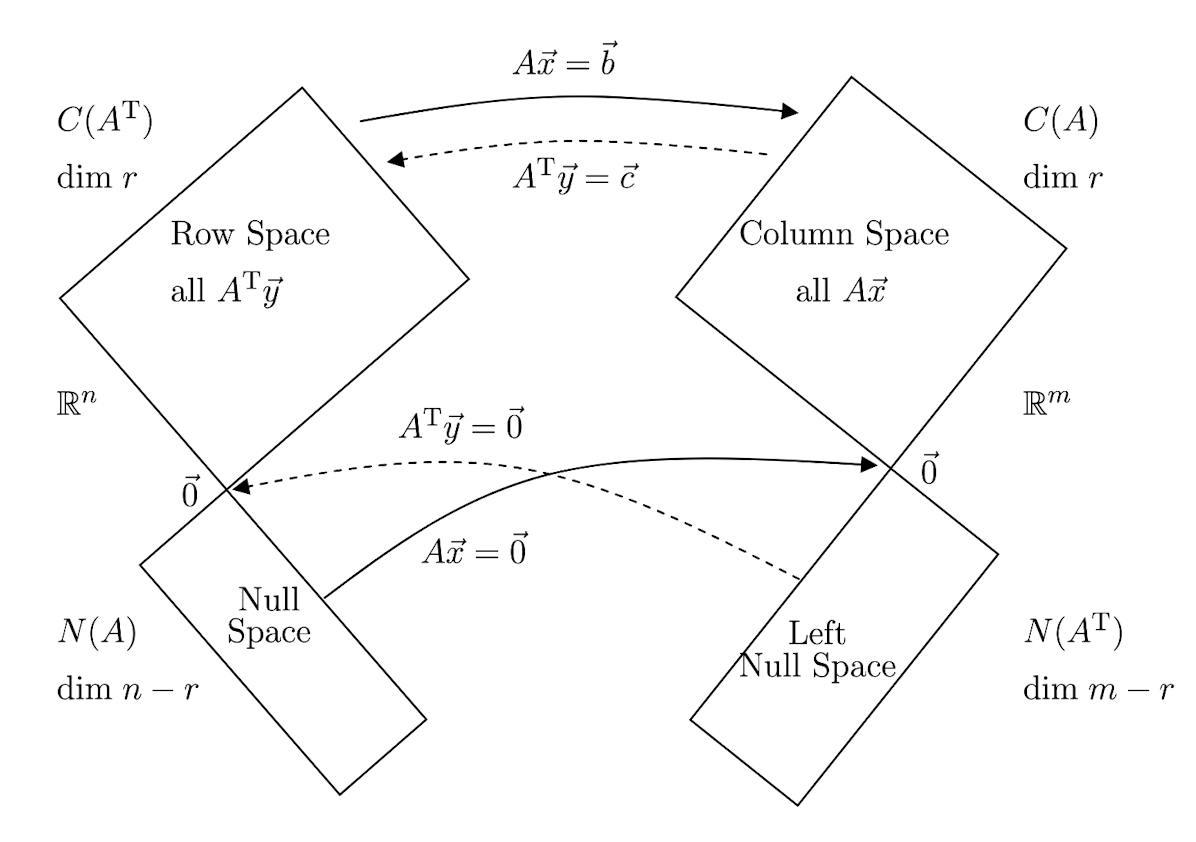
\includegraphics[width=0.75\textwidth]{Figures/grah.png}
    \caption{Fundamental Theorem of Linear Algebra}
\end{figure}

\newpage

\begin{eg}
    Find out the basis for the four fundamental subspaces of the matrix
    \[
        A = \begin{pmatrix}
            1 & 0 & 1 & 0 \\
            2 & 3 & 4 & 1 \\
            4 & 3 & 6 & 1
        \end{pmatrix} \quad \longrightarrow \quad U = \begin{pmatrix}
            \redbox{1} & 0 & 1 & 0 \\
            0 & \redbox{1} & 2/3 & 1/3 \\
            0 & 0 & 0 & 0
        \end{pmatrix} \quad r = 2
    \]
\end{eg}

\begin{enumerate}[label=$\arabic*^\circ$]
    \item $\mathcal{C}(A)$
        \[
            \mathcal{B} = \left\{
                \begin{pmatrix}
                    1 \\ 2 \\ 4
                \end{pmatrix},
                \begin{pmatrix}
                    0 \\ 3 \\ 3
                \end{pmatrix}
            \right\} \quad \dim(\mathcal{C}(A)) = r = 2
        \]

    \item $\mathcal{N}(A)$
    \[
        Ax = 0 \longrightarrow Ux = 0 \longrightarrow U \begin{pmatrix}
            x_1 \\ x_2 \\ x_3 \\ x_4
        \end{pmatrix} = \begin{pmatrix}
            0 \\ 0 \\ 0
        \end{pmatrix}
    \]
    
    \[
        \begin{cases}
            x_1 + x_3 = 0 \\
            x_2 + \frac{2}{3} x_3 + \frac{1}{3} x_4 = 0
        \end{cases}
    \]
    \begin{enumerate}[label=(\alph*)]
        \item $x_3 = 1$, $x_4 = 0$ $\longrightarrow \begin{pmatrix}
            -1 \\ -2/3 \\ 1 \\ 0
        \end{pmatrix} = v_2$
        \item $x_3 = 0$, $x_4 = 1$ $\longrightarrow \begin{pmatrix}
            0 \\ -1/3 \\ 0 \\ 1
        \end{pmatrix} = v_2$
    \end{enumerate}
    Hence, $\mathcal{B} = \mathcal{N}(A)$ is $\{v_1, v_2\}$ and $$\red{\dim(\mathcal{N}(A)) = n - r = 4 - 2 = 2}$$

    \item $\mathcal{C}(A^T)$
    \[
        U = \begin{pmatrix}
            1 & 0 & 1 & 0 \\
            0 & 1 & 2/3 & 1/3 \\
            0 & 0 & 0 & 0
        \end{pmatrix} = \begin{pmatrix}
            S_1 \\ S_2 \\ 0
        \end{pmatrix} \quad \longrightarrow \quad \mathcal{B} = \{S_1^{\red{T}}, S_2^{\red{T}}\}, \quad \red{\dim(\mathcal{C}(A^T)) = r = 2}
    \]
    \item $\mathcal{N}(A^T) \longrightarrow \mathcal{N}(B)$
    \[
        B = \begin{pmatrix}
            1 & 2 & 4 \\
            0 & 3 & 3 \\
            1 & 4 & 6 \\
            0 & 1 & 1
        \end{pmatrix} = A^T \quad \longrightarrow \quad \begin{pmatrix}
            \redbox{1} & 2 & 4 \\
            0 & \redbox{1} & 1 \\
            0 & 0 & 0 \\
            0 & 0 & 0
        \end{pmatrix} \begin{pmatrix}
            y_1 \\ y_2 \\ y_3
        \end{pmatrix} = \begin{pmatrix}
            0 \\ 0 \\ 0 \\ 0
        \end{pmatrix} \quad \longrightarrow \quad
        \begin{cases}
            y_1 + 2y_3 = 0 \\
            y_2 + y_3 = 0
        \end{cases}
    \]
    \[
        z = 1 \longrightarrow \begin{pmatrix}
            -2 \\ -1 \\ 1
        \end{pmatrix} \quad \therefore \mathcal{B} = \left\{
            \begin{pmatrix}
                -2 \\ -1 \\ 1
            \end{pmatrix}
        \right\}, \quad \red{\dim(\mathcal{N}(A^T)) = m - r = 3 - 2 = 1}
    \]
    Check orthogonality
\end{enumerate}

\begin{proposition}[2Q]
    We can find the existence and uniqueness of solution of $Ax=b$.
    \begin{itemize}
        \item \textbf{Existence} of inverse: \\
        The system $Ax=b$ has at least one solution $x$ for each $b$ iff the columns span $\mathbb{R}^m\ (r = \blue{m})$. In this case, $$\exists\; n \times m \text{ ``right'' inverse } C \ni AC = I$$ This is possible only if $m \leq n$.
        \item \textbf{Uniqueness} of inverse: \\
        The system $Ax=b$ has at most one solution $x$ for each $b$ iff the columns are independent $(r = \blue{n})$. In this case, $$\exists\; n \times m \text{ ``left'' inverse } B \ni BA = I$$ This is possible only if $m \geq n$.
    \end{itemize}
\end{proposition}
\begin{proof}
    We separetely prove the two parts.
    \begin{itemize}
        \item \textbf{Existence}: 
        \[
            Ax = b \text{ has a solution for each } b \ \iff \ b \in \mathcal{C}(A), \forall b \in \mathbb{R}^m \ \implies \ \mathcal{C}(A) = \mathbb{R}^m
        \]
        Let $e_1, e_2, \cdots, e_m$ be the standard basis of $\mathbb{R}^m$.

        \vspace{0.5em}

        Then $\exists\; x_1, x_2, \cdots, x_m \ni Ax_i = e_i, \forall i = 1, 2, \cdots, m$

        \vspace{0.5em}

        Let $C = (x_1 \mid x_2 \mid \cdots \mid x_m)$, then $AC = A(x_1 \mid x_2 \mid \cdots \mid x_m) = (e_1 \mid e_2 \mid \cdots \mid e_m) = I_m$.
        \item \textbf{Uniqueness}: 
        \[
            Ax = b \text{ has at most one solution for each } b \in \mathbb{R}^m
        \]
        \[
            \iff \ \forall b \in \mathbb{R}^m, \text{if $b$ can be represented as linear combination of columns of $A$, then it is unique}
        \]
    \end{itemize}
    Hence, proof is complete.
\end{proof}

\begin{eg}
    \[
        A = \begin{pmatrix}
            4 & 0 & 0 \\
            0 & 5 & 0
        \end{pmatrix}_{2 \times 3} \quad m=2, n=3, r = 2 \quad \longrightarrow \quad \exists\; \text{right inverse } C \ni AC = I
    \]
\end{eg}
\begin{enumerate}[label=$\arabic*^\circ$]
    \item \[
        AC = \begin{pmatrix}
            4 & 0 & 0 \\
            0 & 5 & 0
        \end{pmatrix} \begin{pmatrix}
            1/4 & 0 \\
            0 & 1/5 \\
            c_{31} & c_{32}
        \end{pmatrix} = I_2 \quad \implies \quad C \text{ is not unique}
    \]
    \item \[
        \begin{pmatrix}
            1/4 & 0 \\
            0 & 1/5 \\
            c_{31} & c_{32}
        \end{pmatrix} \begin{pmatrix}
            4 & 0 & 0 \\
            0 & 5 & 0
        \end{pmatrix} = \begin{pmatrix}
            1 & 0 & 0 \\
            0 & 1 & 0 \\
            0 & 0 & 1
        \end{pmatrix} \quad \text{\red{impossible} since LHS is } 3 \times 2
    \]
    \item \[
        A_2 = \begin{pmatrix}
            4 & 0 \\
            0 & 5 \\
            0 & 0
        \end{pmatrix}_{3 \times 2} \quad m=3, n=2, r=2 \quad \longrightarrow Ax = b \quad \begin{pmatrix}
            4 & 0 \\
            0 & 5 \\
            0 & 0
        \end{pmatrix} \begin{pmatrix}
            x_1 \\ x_2
        \end{pmatrix} = \begin{pmatrix}
            b_1 \\ b_2 \\ b_3
        \end{pmatrix}
    \]
\end{enumerate}

\newpage

\begin{note}
    The following statements about a square matrix $A_{n \times n}$ are equivalent:
    \begin{enumerate}[label=(\arabic*)]
        \item $A$ is nonsingular (invertible)
        \item The columns of $A$ span $\blue{\mathbb{R}^n}$, so $Ax = b$ has \blue{only one} solution $\forall b \in \mathbb{R}^n$
        \item The columns of $A$ are independent, so $Ax = 0$ has \blue{only one trivial solution $x=0$}
        \item The rows of $A$ span $\blue{\mathbb{R}^n}$
        \item The rows of $A$ are independent
        \item Elimination can be completed: $PA = LDU$ with all $d_i\, \red{\neq}\, 0$
        \item $\exists\; A^{-1} \ni AA^{-1} = A^{-1}A = I_n$
        \item Determinant of $A$ $\det(A)\, \red{\neq}\, 0$
        \item Zero is NOT an eigenvalue of $A$
        \item $A^TA$ is \redbox{positive definite} (\red{正定})
    \end{enumerate}
\end{note}

\section{Graph and Network}
skip

\section{Linear Transformation}
We have seen that a matrix move subspaces around. For example, $A$ maps $\mathcal{N}(A)$ to the \blue{zero vector} and move all vectors into its \blue{column space} $\mathcal{C}(A)$. Let $A$ be an $n \times n$ matrix and $x \in \mathbb{R}^n$, so $A$ transforms $x$ into \blue{$Ax \in \mathcal{C}(A)$}.

\subsection{Notation of Linear Transformation}

\begin{eg}
    Here are some examples of linear transformations:
    \begin{enumerate}[label=$\arabic*^\circ$]
        \item 
        \[
            A = \begin{pmatrix}
                c & 0 \\
                0 & c
            \end{pmatrix} \quad A\begin{pmatrix}
                x_1 \\ x_2
            \end{pmatrix} = \begin{pmatrix}
                cx_1 \\ cx_2
            \end{pmatrix} = c \begin{pmatrix}
                x_1 \\ x_2
            \end{pmatrix} \quad \text{(scaling by $c$)}
        \]
        \item 
        \[
            A = \begin{pmatrix}
                0 & -1 \\
                1 & 0
            \end{pmatrix} \quad A\begin{pmatrix}
                x_1 \\ x_2
            \end{pmatrix} = \begin{pmatrix}
                -x_2 \\ x_1
            \end{pmatrix} \quad \text{(rotation by $90^\circ$)}
        \]
        \item 
        \[
            A = \begin{pmatrix}
                0 & 1 \\
                1 & 0
            \end{pmatrix} \quad A\begin{pmatrix}
                x_1 \\ x_2
            \end{pmatrix} = \begin{pmatrix}
                x_2 \\ x_1
            \end{pmatrix} \quad \text{(reflection about $x_1 = x_2$)}
        \]
        \item 
        \[
            A = \begin{pmatrix}
                1 & 0 \\
                0 & 0
            \end{pmatrix} \quad A\begin{pmatrix}
                x_1 \\ x_2
            \end{pmatrix} = \begin{pmatrix}
                x_1 \\ 0
            \end{pmatrix} \quad \text{(projection onto $x_1$-axis)}
        \]
    \end{enumerate}
\end{eg}

\newpage
